\begin{tikzpicture}
  \pgfdeclarelayer{back}
  \pgfsetlayers{back,main}
  \setlength{\unit}{1.8cm}

  \colorlet{model}{yellow!70!red};
  \colorlet{irf}{blue!60!red};


  \tikzset{%
    con/.style={-{Triangle[length=0.25cm, width=0.3cm]}, line width=0.1\unit},
    ana/.style={text width=\unit, text=white, align=center, anchor=west, minimum height=0.25\unit},
    zlevel/.style={%
      execute at begin scope={\pgfonlayer{#1}},
      execute at end scope={\endpgfonlayer}
    },
  }

  \node[ana, align=right] (source) at (0.5\unit, 1.5\unit) {%
    \tiny%
    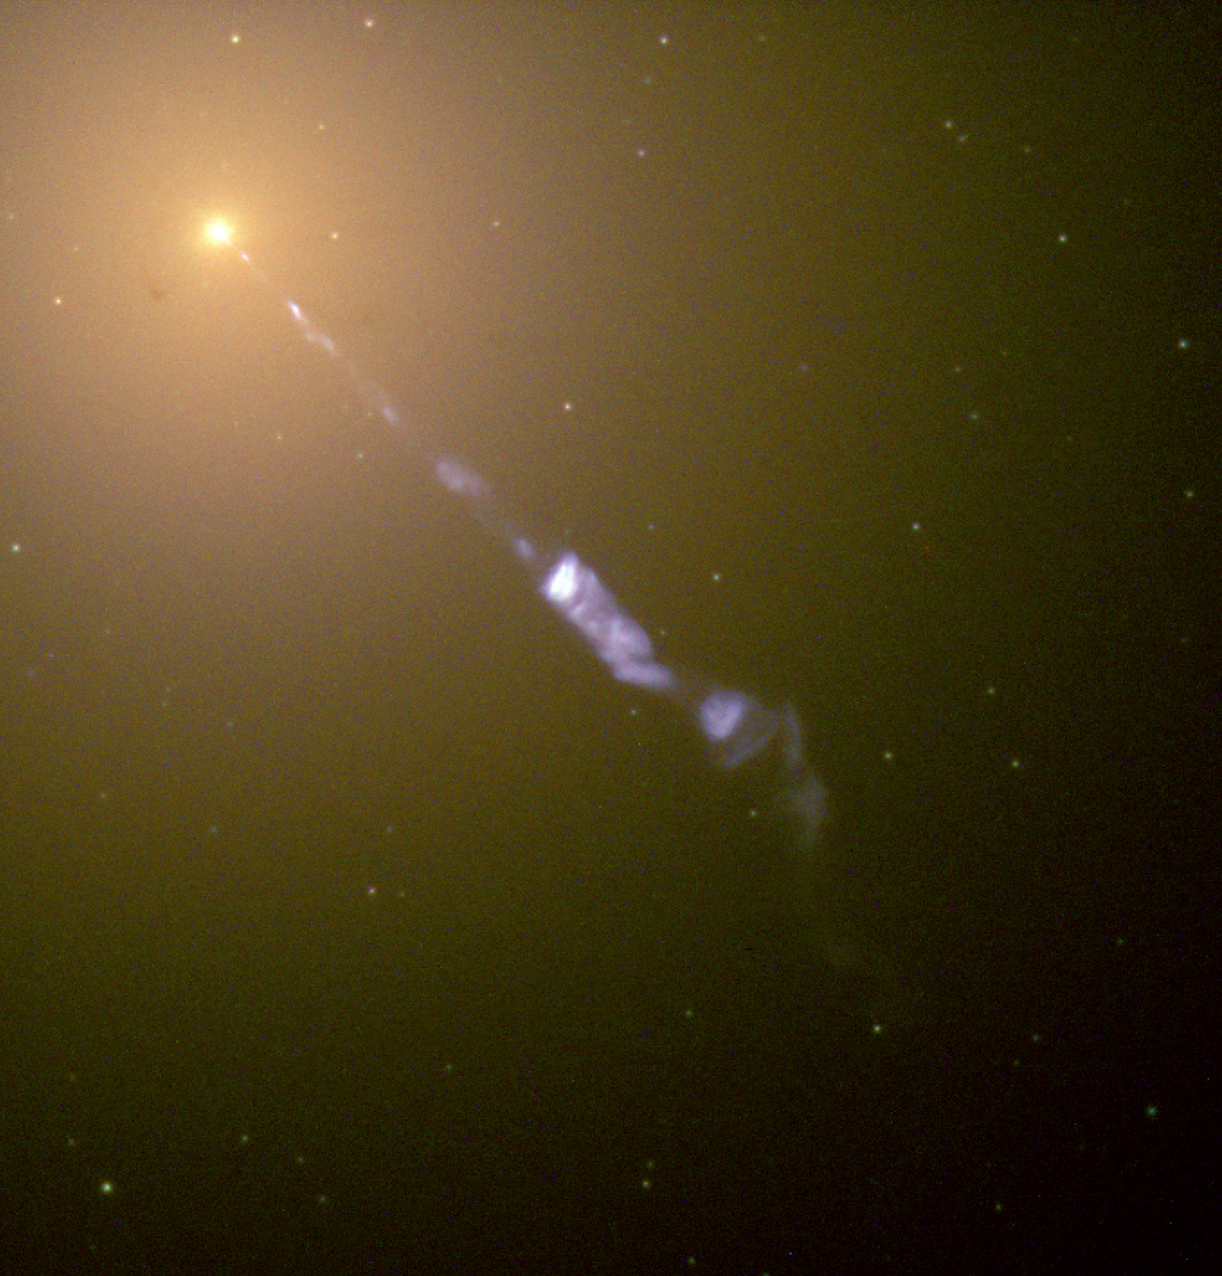
\includegraphics[height=1\unit]{../thesis/images/m87.jpg}\\[-2\baselineskip]
    \color{white}NASA/STSI
  };

  \node[ana, align=right] (atmosphere) at (0.5\unit, 0) {%
    \tiny%
    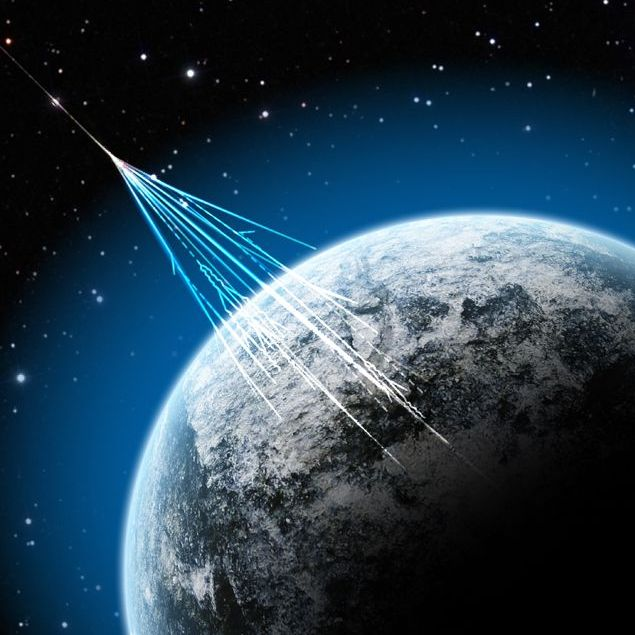
\includegraphics[height=1\unit]{images/airshower.jpg}\\[-2\baselineskip]
    \color{white}NSF/Yang
  };

  \draw[con, darkgray] (source.south) -- (atmosphere.north); 

  \node[anchor=west, text width=\unit, align=center, text opacity=1] (telescope) at (2\unit, 0) {
    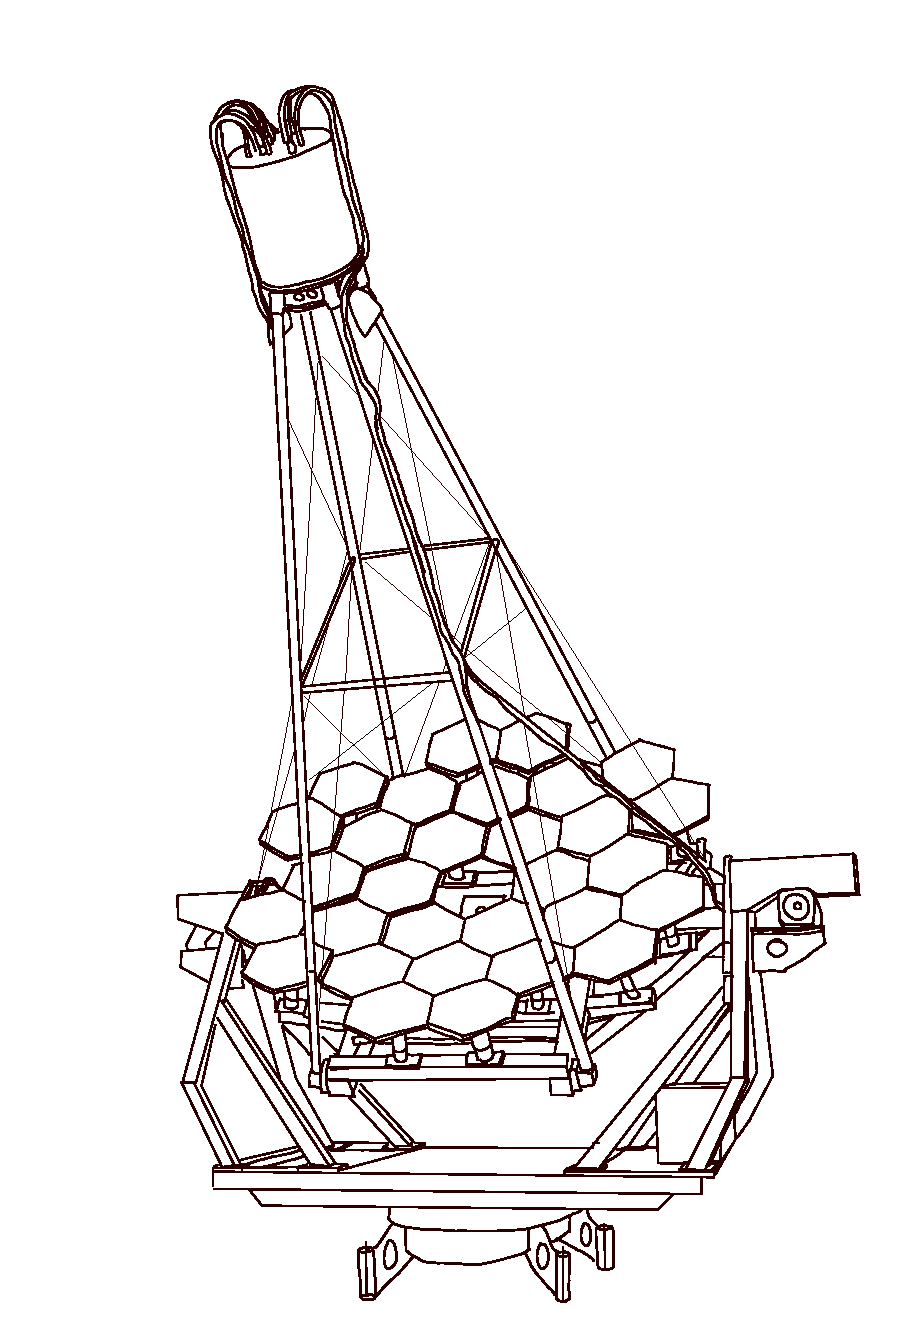
\includegraphics[width=1\unit]{images/fact_sketch.pdf}
  };


  \draw[con, darkgray] (atmosphere.east) -- (telescope.west); 
  \node[ana, fill=darkgray] (obs) at (5.5\unit, 0) {Observationen};
  \draw[con] (telescope.east) -- (obs.west);  

  \onslide<2->{
    \node[ana] (corsika) at (0.5\unit, -1.5\unit) {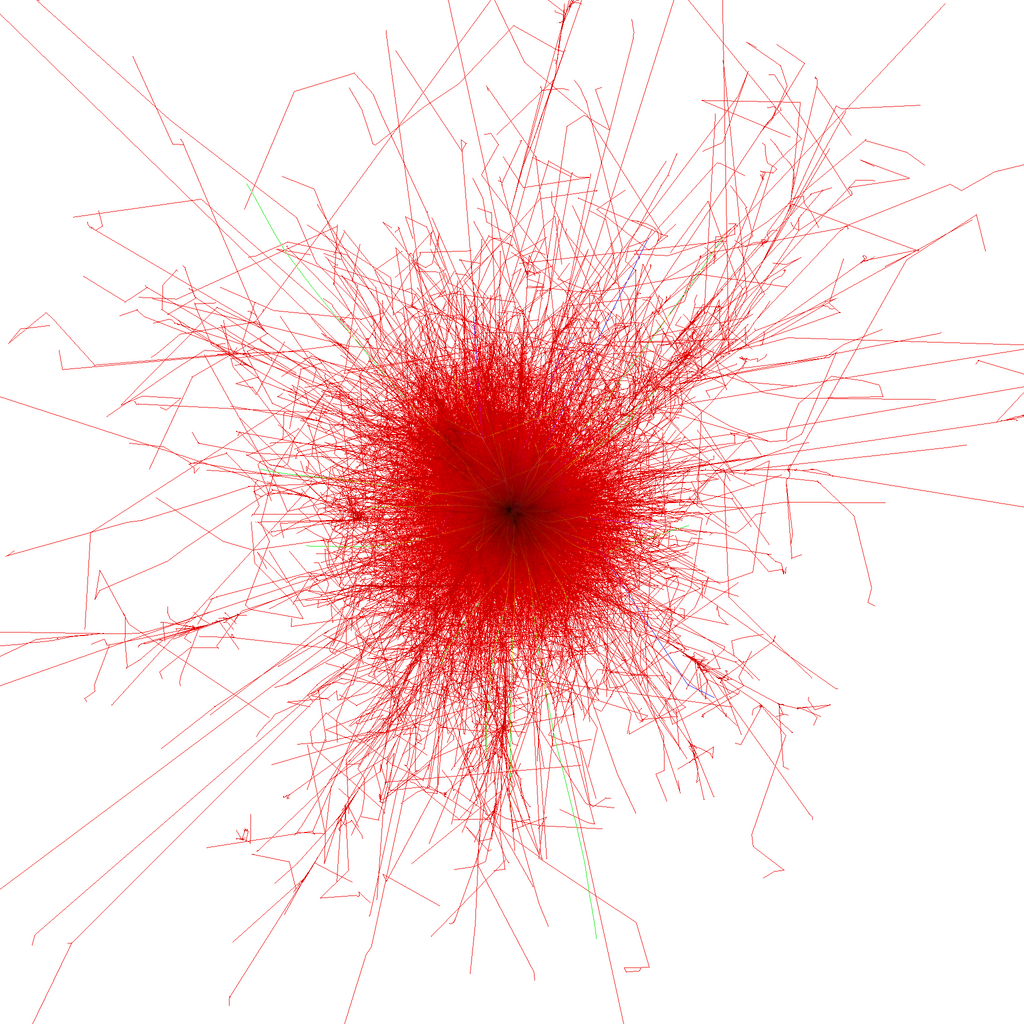
\includegraphics[width=\unit]{images/proton_12_0deg.xy.png}};
    \node[ana, anchor=center, text width=1.1\unit, yshift=-0.25\unit] at (corsika.center) {\huge\color{black} CORSIKA};

    \node[ana] (ceres) at (2\unit, -1.5\unit) {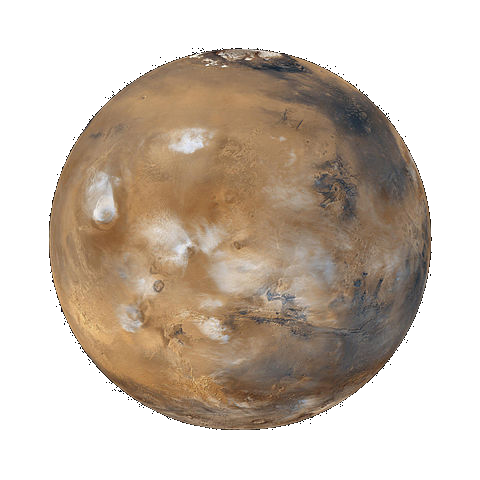
\includegraphics[width=\unit]{images/mars_trim.png}};
    \node[ana, fill=white, opacity=0.6, text opacity=1, yshift=-0.25\unit, anchor=center] at (ceres.center) {\huge\color{black} CERES};
    \draw[con, gamma] (corsika.15) -- (ceres.165);
    \draw[con, proton] (corsika.345) -- (ceres.195);

    \node[ana, fill=gamma] (diffus) at (3.75\unit, -1\unit) {$\symup{\gamma}$, diffus};
    \node[ana, fill=gamma] (pointlike) at (3.75\unit, -2\unit) {$\symup{\gamma}$, punkt.};
    \node[ana, fill=proton] (proton) at (3.75\unit, -1.5\unit) {p, diffus};

    \draw[con, proton] (ceres.east) to[out=0, in=180] (proton.west);  
    \draw[con, gamma] (ceres.east) to[out=0, in=180] (diffus.west);  
    \draw[con, gamma] (ceres.east) to[out=0, in=180] (pointlike.west);  
  }

  \onslide<3-> {


    \node[ana, fill=model] (ml) at (5.5\unit, -0.75\unit) {ML-Modelle}; 

    \node[ana, fill=proton] (ptrain) at (5.5\unit, -1.35\unit) {p, Training};
    \node[ana, fill=proton] (ptest) at (7\unit, -1.65\unit) {p, Test};

    \node[ana, fill=gamma] (gtrain) at (5.5\unit, -1.85\unit) {\pGamma{}, Training};
    \node[ana, fill=gamma] (gtest) at (7\unit, -2\unit) {\pGamma{}, Test};

    \begin{pgfonlayer}{back}
      \onslide<3->{
        \draw[con, gamma] (gtrain.150) -- (ml.210);
      }
    \end{pgfonlayer}

    \draw[con, proton, line width=0.02\unit] (proton.east) to[out=0, in=180] (ptrain.west);

    \coordinate (tmp) at (5.5\unit, -1.65\unit);
    \draw[con, proton, line width=0.08\unit] (proton.east) to[out=0, in=180] (tmp) -- (ptest.west);


    \draw[con, proton] (ptrain.north) -- (ml.south);
    \draw[con, gamma] (diffus.east) to[out=0, in=180] (ml.west);

    \coordinate (tmp1) at (5.5\unit, -2.15\unit);
    \coordinate (tmp2) at (6.5\unit, -2.15\unit);
    \draw[con, gamma, line width=0.08\unit] (pointlike.east) to[in=180, out=0] (tmp1) to[in=180, out=0] (tmp2) to[in=180, out=0](gtest.west);

    \draw[con, gamma, line width=0.02\unit] (pointlike.east) to[in=180, out=0] (gtrain.west);

  }
  \onslide<4->{
    \draw[con, model] (ml.north) -- (obs.south);

    \begin{pgfonlayer}{back}
      \onslide<4->{
        \fill[darkgray] ($ (ptest.north west) + (-0.1\unit, 0.1\unit)$) rectangle ($(gtest.south east) + (0.1\unit, -0.1\unit)$);
      }
    \end{pgfonlayer}

    \draw[con, model] (ml.east) to[out=0, in=90] ($(ptest.north) + (-0.33333\unit, 0.1\unit)$);

    \node[ana, fill=irf] (irf) at (7\unit, 0) {Detektorantwort};
    \draw[con, darkgray] ($(ptest.north) + (0, 0.1\unit)$) -- (irf.south);

    \node[ana, fill=irf] (sens) at (7\unit, 1\unit) {Sensitivität};
    \node[ana, fill=irf] (spec) at (7\unit, 0.7\unit) {Spektrum};
    \draw[con, darkgray] (obs.north) to[out=90, in=180] (sens.west); 
    \draw[con, darkgray] (obs.north) to[out=90, in=180] (spec.west); 
    \draw[con, irf] (irf.north) -- (spec.south); 

    \coordinate (tmp) at (8.7\unit, -0.3\unit);
    \draw[con, darkgray] ($(ptest.south) + (0.6\unit, -0.05\unit)$) to[out=0, in=270]  (tmp) to[out=90, in=0]  (sens.east);
  }
\end{tikzpicture}
